This section provides information on the structure of the classes are build around Spotify Web API [AND POSSIBLY THE WHOLE PROJECT]. It will describe the considerations and approaches that has been taken, when designing the architecture.

When using the Web API to search on Spotify, three different items can be found Track, Album and Artist. These three items are all identified by a unique ID from Spotify, which is what is also used as the id for the item in this project. A small problem occurs in the implementation of this search since it is required to specify what kind of item is being searched for. The user, although always eventually looking for a track, does not always find the track directly via the title, but often via the artist by whom it was created or album on which the track is placed. It was therefore chosen that each search requires a specification on what type item that is being searched for. To minimize the requirements for the user, it was decided that the user, should not specify what item they are searching, but rather they should write the search string, and get a complete list of the results for all items represented. Therefore it has been implemented, that it is possible, when creating a Search object, to specify from an enum which of the three items or all three are being searched for. When choosing all three, which is what is done for the users searches, three individual searches are created and the results are represented in a complete structure shown in \cref{fig:WebAPIUML}.

\begin{figure}[H]
\centering
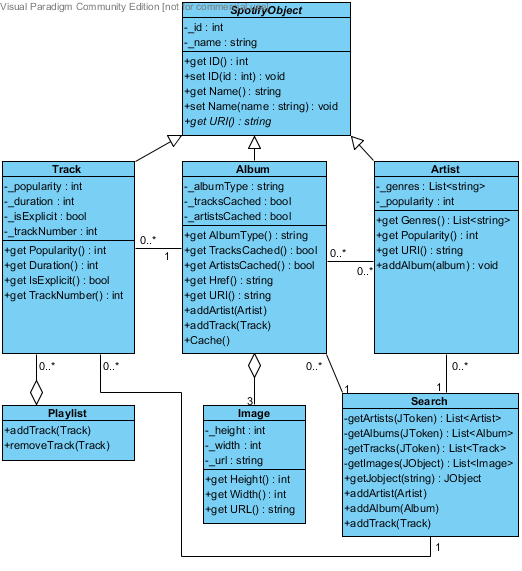
\includegraphics[width=\textwidth]{Images/WebAPIUML.png}
\caption{A class diagram showing the class structure of the results generated from a search}
\label{fig:WebAPIUML}
\end{figure}

It was decided to have a minimal data download approach when designing the web API. This was done on the bases of the assumption that this API would most likely be the system used for searching for new tracks on the mobile front-end application. Since mobile phones still have limited data access, it is preferable for the user to use as little data as possible. This approach results in only three searches being done, one for each item type. Other requests are not done until other information about the item is needed. Furthermore this approach also results in all information being stored in the objects locally. It will be saved until the search object is removed, and the user hopefully has found his or her track.

One search usually searches for all three different item types, track, album and artist, and present these to the user. Not all information about the artists and albums can be gathered from the json code received from these three initial searches. Albums does not have information about it tracks nor its artists initially, and an artist does not have information about its albums. The minimal data approach was therefore combined with another idea, data just in time. This was done since the user normally only wants information from one type of item, and not the two remaining types. It would therefore be undesirable for the user to wait, for all information for every item to be downloaded. This also fits very well with the minimal data approach since this minimize the amount of data requested, if the user does not look though all items in the search. The information not received from the initial searches, is therefore only requested from Spotify when the get method for the properties on items are called. To keep faithful to the minimal data approach this information is cached to the application and saved in the object structure so that the data does not have to be downloaded again.
